\documentclass[11pt]{article}
% ─────────────────────────────────────────────────────────────────────────────
% ตั้งค่าเอกสารภาษาไทย สำหรับ XeLaTeX
%
% ทำไมต้อง XeLaTeX ไม่ใช่ pdfLaTeX:
%   pdfLaTeX จัดการ Unicode และฟอนต์ระบบไม่ได้ ภาษาไทยจึงต้องใช้ XeLaTeX หรือ LuaLaTeX
%
% ทำไมต้อง \XeTeXlinebreaklocale:
%   ภาษาไทยไม่เว้นวรรคระหว่างคำ ถ้าไม่บอก TeX ว่าเป็นภาษาไทย
%   มันจะไม่ยอมตัดบรรทัดเลย ทำให้ข้อความล้นออกนอกหน้ากระดาษ
% ─────────────────────────────────────────────────────────────────────────────

\usepackage{fontspec}
\usepackage[a4paper,margin=2.4cm,bottom=2.6cm]{geometry}
\usepackage{graphicx}
\usepackage{booktabs}
\usepackage{xcolor}
\usepackage{enumitem}
\usepackage{titlesec}
\usepackage{fancyhdr}
\usepackage{caption}
\usepackage[most]{tcolorbox}
\usepackage{amsmath}
\usepackage[hidelinks]{hyperref}

% ----------------------------------------------------
%  ฟอนต์
%
%  ใช้ฟอนต์ตระกูล TLWG ซึ่งมีทั้งอักขระไทยและละตินอยู่ในไฟล์เดียวกัน
%  จงใจเลือกแบบนี้แทนการจับคู่ Noto Serif (ละติน) กับ Noto Serif Thai
%  เพราะ Noto Serif Thai ไม่มีอักขระละตินเลย การผสมสองฟอนต์จึงต้องพึ่ง
%  ucharclasses ซึ่งสลับฟอนต์ตาม "บล็อกยูนิโคด" ที่เจอ ปัญหาคือมันไม่รู้จัก
%  ขอบเขตของกลุ่ม TeX ดังนั้นข้อความละตินที่ตามหลังกลุ่มอย่าง \textbf{...}
%  จะยังติดฟอนต์ไทยและหายไปทั้งหมด ทั้งยังชนกับ titlesec จนคอมไพล์ไม่ผ่าน
%  ฟอนต์สองสคริปต์ในไฟล์เดียวตัดปัญหานี้ทิ้งทั้งชุด
%
%    Laksaman — ไทยไม่มีหัว + ละตินตัวไม่มีเชิง อ่านง่ายที่สุดสำหรับเนื้อความ
%    Garuda   — ตัวไม่มีเชิงที่หนากว่า ใช้กับหัวข้อและป้ายในไดอะแกรม
%    Tlwg Mono — ความกว้างคงที่จริง ใช้กับชื่อไฟล์และโค้ด
% ----------------------------------------------------

\setmainfont{Laksaman}
\setsansfont{Garuda}
\newfontfamily\thaimono{Tlwg Mono}

\XeTeXlinebreaklocale "th"
\XeTeXlinebreakskip = 0pt plus 0.15pt

% ─── สี ───
\definecolor{ink}{HTML}{1A1A1A}
\definecolor{accent}{HTML}{C0392B}
\definecolor{blue}{HTML}{2C5AA0}
\definecolor{soft}{HTML}{F4F6F8}
\definecolor{warnbg}{HTML}{FDF3F2}
\definecolor{keybg}{HTML}{EEF3FA}
\definecolor{grey}{HTML}{6B7280}

\color{ink}

% ─── หัวข้อ ───
\titleformat{\section}{\sffamily\Large\bfseries\color{blue}}{\thesection}{0.6em}{}
\titleformat{\subsection}{\sffamily\large\bfseries}{\thesubsection}{0.6em}{}
\titlespacing*{\section}{0pt}{2.2ex plus 1ex minus .2ex}{1.2ex plus .2ex}

\setlist[itemize]{leftmargin=1.3em,itemsep=0.25ex,topsep=0.5ex}
\setlist[enumerate]{leftmargin=1.5em,itemsep=0.25ex,topsep=0.5ex}

\captionsetup{font=small,labelfont={bf,color=blue},skip=4pt}

\pagestyle{fancy}
\fancyhf{}
\fancyhead[L]{\small\sffamily\color{grey}\leftmark}
\fancyfoot[C]{\small\thepage}
\renewcommand{\headrulewidth}{0.3pt}

% ─── กล่องนิยามศัพท์ ───
%
% toptitle เผื่อที่ไว้ด้านบนของแถบหัวกล่อง เพราะ tcolorbox คิดความสูงจาก
% ระยะขึ้น-ลงของอักษรละติน ซึ่งไม่เผื่อวรรณยุกต์และสระบนของไทยที่ซ้อนสูงกว่า
% ถ้าไม่ใส่ ไม้โท/ไม้ไต่คู้ในหัวข้อจะถูกตัดบน
\newtcolorbox{term}[1]{
  colback=keybg, colframe=blue, boxrule=0.7pt, arc=2pt,
  left=8pt, right=8pt, top=6pt, bottom=6pt,
  toptitle=3pt, bottomtitle=1pt,
  title={\sffamily\bfseries #1}, coltitle=white, fonttitle=\small,
  breakable
}

% ─── กล่องคำเตือน / กับดัก ───
\newtcolorbox{trap}[1]{
  colback=warnbg, colframe=accent, boxrule=0.7pt, arc=2pt,
  left=8pt, right=8pt, top=6pt, bottom=6pt,
  toptitle=3pt, bottomtitle=1pt,
  title={\sffamily\bfseries #1}, coltitle=white, fonttitle=\small,
  breakable
}

% ─── กล่องสรุปประเด็นสำคัญ ───
\newtcolorbox{keypoint}{
  colback=soft, colframe=grey!45, boxrule=0.5pt, arc=2pt,
  left=8pt, right=8pt, top=6pt, bottom=6pt,
  breakable
}

% ─── ตัวช่วยเล็ก ๆ ───
\newcommand{\eng}[1]{\textsf{#1}}
\newcommand{\code}[1]{{\thaimono\small #1}}
\newcommand{\figref}[1]{รูปที่~\ref{#1}}

% เปลี่ยนคำที่ LaTeX ใส่ให้เองเป็นภาษาไทย
% (ปกติ polyglossia จัดการให้ แต่ที่นี่ใช้แค่ไม่กี่คำจึงเปลี่ยนตรง ๆ ง่ายกว่า)
\renewcommand{\contentsname}{สารบัญ}
\renewcommand{\figurename}{รูปที่}
\renewcommand{\tablename}{ตารางที่}


\title{}
\date{}

\begin{document}

% ═══════════════════════════════════════════════════════════════════════════
\begin{titlepage}
\centering
\vspace*{3cm}

{\sffamily\Huge\bfseries\color{blue} จากศูนย์ถึงโปรเจกต์\par}
\vspace{0.8cm}
{\sffamily\LARGE หุ้น การเทรด และการลงทุนเชิงปริมาณ\par}
\vspace{0.4cm}
{\sffamily\large\color{grey} อธิบายสำหรับคนที่ไม่เคยลงทุนมาก่อนเลย\par}

\vspace{2.5cm}
\rule{0.55\textwidth}{0.4pt}

\vspace{1.2cm}
\begin{minipage}{0.78\textwidth}
\centering\small
เอกสารนี้อธิบายทุกอย่างตั้งแต่ ``หุ้นคืออะไร'' ไปจนถึงเหตุผลเบื้องหลัง
การตัดสินใจออกแบบทุกข้อในโปรเจกต์ \code{finbg}

\vspace{0.5em}
กราฟทุกรูปสร้างจากข้อมูลตลาดจริงที่โปรเจกต์เก็บไว้เอง
ไม่ได้ดึงภาพจากอินเทอร์เน็ต
\end{minipage}

\vfill
{\small\color{grey} 6 สิงหาคม 2026\par}
\end{titlepage}

\tableofcontents
\newpage

% ═══════════════════════════════════════════════════════════════════════════
\section{ทำไมต้องอ่านเอกสารนี้}
\markboth{ทำไมต้องอ่านเอกสารนี้}{}

โปรเจกต์นี้โตขึ้นเร็วมากในไม่กี่วัน มีทั้งคำว่า \eng{point-in-time}, \eng{hindsight},
\eng{cross-sectional}, \eng{materiality}, \eng{factor} ปนกันจนตามไม่ทัน
เอกสารนี้จึงถอยกลับไปเริ่มที่จุดเริ่มต้นจริง ๆ แล้วค่อย ๆ ต่อขึ้นมา

โครงสร้างเป็นแบบนี้

\begin{keypoint}
\textbf{บทที่ 2--3} \quad พื้นฐานที่สุด --- หุ้นคืออะไร ราคาเกิดจากอะไร คำศัพท์ที่ต้องรู้\\
\textbf{บทที่ 4} \quad ความจริงที่ขัดกับสัญชาตญาณ --- สิ่งที่คนส่วนใหญ่เข้าใจผิด\\
\textbf{บทที่ 5--6} \quad \eng{Quant} คืออะไร และกับดักที่ทำให้ผลทดสอบโกหก\\
\textbf{บทที่ 7} \quad AI กับการลงทุน --- อะไรได้ผล อะไรไม่ได้ผล และหลักฐาน\\
\textbf{บทที่ 8--9} \quad โปรเจกต์นี้ทำอะไรอยู่ และแผนงานข้างหน้า\\
\textbf{บทที่ 10} \quad อภิธานศัพท์ --- เปิดหาเวลาเจอคำที่ลืม
\end{keypoint}

ถ้าคุณรู้พื้นฐานอยู่แล้ว ข้ามไปบทที่ 5 ได้เลย
แต่ถ้าคำว่า ``\eng{Sharpe ratio}'' ยังไม่คุ้น แนะนำให้อ่านตามลำดับ

% ═══════════════════════════════════════════════════════════════════════════
\section{หุ้นคืออะไรกันแน่}
\markboth{หุ้นคืออะไรกันแน่}{}

\subsection{ซื้อหุ้นคือซื้ออะไร}

เวลาคุณซื้อหุ้น \eng{Apple} หนึ่งหุ้น คุณกำลังซื้อ \textbf{ความเป็นเจ้าของบริษัทจริง}
เศษเสี้ยวหนึ่ง ไม่ใช่ตั๋วเดิมพันว่าตัวเลขจะขึ้นหรือลง

\eng{Apple} มีหุ้นทั้งหมดราว 15,000 ล้านหุ้น ถ้าคุณถือ 1 หุ้น
คุณเป็นเจ้าของบริษัทนั้นอยู่ 1 ใน 15,000 ล้านส่วน
ซึ่งหมายความว่าคุณมีสิทธิ์ในกำไรของบริษัทตามสัดส่วนนั้นจริง ๆ

ประโยคนี้สำคัญกว่าที่คิด เพราะมันตอบว่า
\textbf{ทำไมตลาดหุ้นถึงให้ผลตอบแทนเป็นบวกในระยะยาว} --- ไม่ใช่เพราะมีคนมาซื้อต่อในราคาแพงกว่า
แต่เพราะบริษัทข้างหลังมันสร้างกำไรเพิ่มขึ้นเรื่อย ๆ จริง

\begin{term}{มูลค่าตลาด (\eng{Market Capitalization})}
ราคาต่อหุ้น $\times$ จำนวนหุ้นทั้งหมด $=$ มูลค่าของทั้งบริษัทตามที่ตลาดประเมิน

ถ้าหุ้นราคา \$200 และมี 15,000 ล้านหุ้น มูลค่าตลาดคือ \$3 ล้านล้าน
\end{term}

\subsection{ราคาเกิดขึ้นได้อย่างไร}

หลายคนคิดว่ามี ``ใครสักคน'' กำหนดราคาหุ้น ความจริงคือไม่มี
ราคาเกิดจากการที่คนซื้อกับคนขายมาเจอกันเท่านั้น

ในตลาดจริงจะมีสิ่งที่เรียกว่า \textbf{สมุดคำสั่ง} (\eng{order book}) หน้าตาแบบนี้

\begin{center}
\small
\begin{tabular}{rl@{\hspace{2.5em}}rl}
\toprule
\multicolumn{2}{c}{\textbf{คนอยากซื้อ} (\eng{bid})} & \multicolumn{2}{c}{\textbf{คนอยากขาย} (\eng{ask})} \\
\midrule
\$199.98 & 400 หุ้น & \$200.02 & 250 หุ้น \\
\$199.97 & 1,200 หุ้น & \$200.03 & 900 หุ้น \\
\$199.95 & 3,000 หุ้น & \$200.05 & 1,500 หุ้น \\
\bottomrule
\end{tabular}
\end{center}

คนที่ยอมจ่ายแพงที่สุดคือ \$199.98 ส่วนคนที่ยอมขายถูกที่สุดคือ \$200.02
ทั้งคู่ยังไม่ตกลงกัน ราคาจึงยังไม่ขยับ

พอมีใครสักคนใจร้อน ยอมซื้อที่ \$200.02 การซื้อขายก็เกิดขึ้น
และ \textbf{นั่นแหละคือ ``ราคาหุ้น'' ที่คุณเห็นบนจอ} --- มันคือราคาของ
\emph{ดีลล่าสุดที่เพิ่งเกิด} ไม่ใช่ราคาที่ใครประกาศไว้

\begin{term}{ส่วนต่างราคาเสนอซื้อ--ขาย (\eng{Bid-Ask Spread})}
ช่องว่างระหว่าง \$199.98 กับ \$200.02 คือ \$0.04

นี่คือ \textbf{ต้นทุนที่คุณจ่ายทันทีที่ซื้อ} เพราะถ้าซื้อแล้วขายคืนเดี๋ยวนั้น
คุณจะขาดทุน \$0.04 ต่อหุ้นโดยที่ราคาไม่ได้ขยับเลย
\end{term}

\subsection{ผลตอบแทนมาจากสองทาง}

\begin{enumerate}
\item \textbf{ส่วนต่างราคา} (\eng{capital gain}) --- ซื้อ \$100 ขาย \$120 ได้กำไร \$20
\item \textbf{เงินปันผล} (\eng{dividend}) --- บริษัทแบ่งกำไรมาให้ผู้ถือหุ้นเป็นเงินสด
\end{enumerate}

ข้อสองสำคัญกว่าที่คนมือใหม่คิด เพราะเวลาดูกราฟราคาเปล่า ๆ
คุณจะเห็นแค่ข้อแรก ทำให้ประเมินผลตอบแทนจริงต่ำกว่าความเป็นจริง

\begin{term}{ราคาปรับแล้ว (\eng{Adjusted Close})}
ราคาปิดที่บวกเงินปันผลกลับเข้าไปแล้ว และปรับผลจากการแตกหุ้น (\eng{stock split})

\textbf{งานวิเคราะห์ทุกชิ้นต้องใช้ราคาปรับแล้วเสมอ} ไม่ใช่ราคาปิดดิบ
ไม่งั้นผลตอบแทนที่คำนวณได้จะต่ำกว่าความจริง และหุ้นที่แตกพาร์จะดูเหมือนราคาตกฮวบ
ทั้งที่ไม่มีอะไรเกิดขึ้น

โปรเจกต์นี้เก็บช่อง \code{adj\_close} ไว้ด้วยเหตุผลนี้
\end{term}

\subsection{หน้าตาจริงของราคาหุ้นระยะยาว}

\begin{figure}[htbp]
\centering
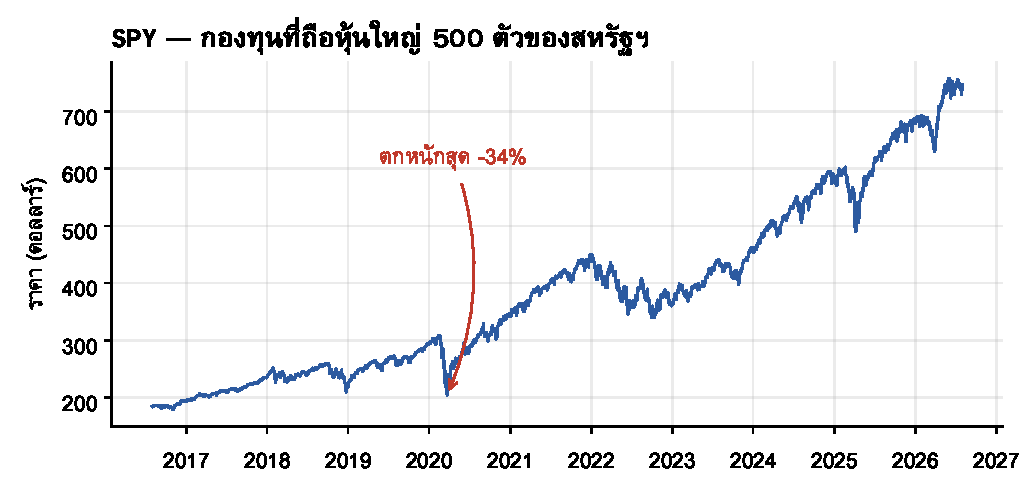
\includegraphics[width=\textwidth]{figures/01-price-history.pdf}
\caption{ราคาของ \eng{SPY} ตลอด 10 ปี --- ข้อมูลจริงจากคลังของโปรเจกต์
(1 ส.ค. 2016 ถึง 31 ก.ค. 2026)}
\label{fig:price}
\end{figure}

\figref{fig:price} คือกราฟของ \eng{SPY} ซึ่งเป็นกองทุนที่ถือหุ้นใหญ่ 500 ตัวของสหรัฐฯ
ตลอด 10 ปีนี้มันให้ผลตอบแทน \textbf{+304\%} หรือประมาณ \textbf{15.0\% ต่อปี}

แต่สังเกตลูกศรสีแดง --- ระหว่างทางมีช่วงที่ราคาตกลงไป \textbf{34\%} จากจุดสูงสุด
ถ้าตอนนั้นคุณมีเงิน 1 ล้านบาทในตลาด มันจะเหลือ 660,000 บาท และคุณไม่รู้เลยว่า
มันจะฟื้นหรือจะตกต่อ

\begin{keypoint}
\textbf{บทเรียนแรกที่สำคัญที่สุด:} ``ผลตอบแทนดีในระยะยาว'' กับ ``ถือได้สบายใจ''
เป็นคนละเรื่องกันอย่างสิ้นเชิง กราฟที่ดูสวยเวลามองย้อนหลัง 10 ปี
คือกราฟที่โหดร้ายมากตอนอยู่ในนั้นจริง ๆ
\end{keypoint}

% ═══════════════════════════════════════════════════════════════════════════
\section{คำศัพท์ที่ต้องรู้ก่อนไปต่อ}
\markboth{คำศัพท์ที่ต้องรู้ก่อนไปต่อ}{}

\subsection{ชื่อย่อ ดัชนี และกองทุนดัชนี}

\begin{term}{\eng{Ticker} --- ชื่อย่อหุ้น}
รหัสสั้น ๆ ที่ใช้แทนหลักทรัพย์แต่ละตัว เช่น \eng{AAPL} คือ \eng{Apple},
\eng{MSFT} คือ \eng{Microsoft}

ในโปรเจกต์นี้ ชื่อย่อคือ \emph{กุญแจ} ที่ใช้เชื่อมข่าวเข้ากับราคา
ถ้าจับชื่อย่อผิด ข้อมูลทั้งชุดก็ผิดตาม --- ซึ่งเคยเกิดขึ้นจริงและจะเล่าในบทที่ 9
\end{term}

\begin{term}{ดัชนี (\eng{Index}) และกองทุนดัชนี (\eng{ETF})}
\textbf{ดัชนี} คือตัวเลขที่วัดภาพรวมของกลุ่มหุ้น เช่น \eng{S\&P 500}
วัดหุ้นใหญ่ 500 ตัวของสหรัฐฯ --- ตัวมันเองซื้อไม่ได้ เป็นแค่ตัวเลข

\textbf{ETF} คือกองทุนที่ซื้อขายได้เหมือนหุ้นตัวเดียว แต่ข้างในถือหุ้นหลายตัว
\eng{SPY} คือ \eng{ETF} ที่ไล่ตาม \eng{S\&P 500} --- ซื้อ \eng{SPY} หนึ่งหุ้น
เท่ากับซื้อหุ้น 500 ตัวพร้อมกันในสัดส่วนที่เหมาะสม
\end{term}

โปรเจกต์นี้เก็บราคาของ \eng{ETF} รายกลุ่มธุรกิจ 11 ตัว (\eng{XLK}, \eng{XLF}, \eng{XLE} \ldots)
เพราะมันเป็นวิธีที่สะอาดที่สุดในการวัดว่า ``กลุ่มเทคโนโลยีไปได้ดีกว่ากลุ่มพลังงานไหม''
โดยไม่ต้องไปยุ่งกับหุ้นรายตัวหลายร้อยตัว

\subsection{ผลตอบแทนและการทบต้น}

ผลตอบแทนรายวันคำนวณง่ายมาก

\[
r_t = \frac{P_t - P_{t-1}}{P_{t-1}}
\]

ถ้าเมื่อวานราคา \$100 วันนี้ \$102 ผลตอบแทนคือ $+2\%$

แต่สิ่งที่คนพลาดบ่อยคือ \textbf{ผลตอบแทนบวกกันตรง ๆ ไม่ได้}

\begin{trap}{กับดัก: $+50\%$ แล้ว $-50\%$ ไม่ได้เท่าทุน}
เริ่มที่ 100 บาท $\rightarrow$ $+50\%$ $\rightarrow$ 150 บาท $\rightarrow$ $-50\%$ $\rightarrow$ \textbf{75 บาท}

คุณขาดทุน 25\% ทั้งที่ผลตอบแทนบวกลบดูเหมือนหักล้างกันพอดี

นี่คือเหตุผลว่าทำไมการ \textbf{ไม่ขาดทุนหนัก} มีค่ามากกว่าการทำกำไรสูง
ถ้าขาดทุน 50\% คุณต้องทำกำไร 100\% แค่จะกลับมาเท่าทุน
\end{trap}

\subsection{ความผันผวน --- ตัววัด ``ความเสี่ยง'' ที่ใช้กันมากที่สุด}

\begin{term}{ความผันผวน (\eng{Volatility})}
ส่วนเบี่ยงเบนมาตรฐานของผลตอบแทน พูดง่าย ๆ คือ ``ปกติแล้วมันเหวี่ยงแรงแค่ไหน''

นิยมรายงานเป็นรายปี โดยคูณค่ารายวันด้วย $\sqrt{252}$
(252 คือจำนวนวันทำการในหนึ่งปี)

\eng{SPY} ในช่วง 10 ปีที่ผ่านมามีความผันผวน \textbf{17.9\% ต่อปี}
แปลว่าในปีทั่ว ๆ ไป ผลตอบแทนจะเบี่ยงจากค่าเฉลี่ยราว $\pm$18\%
\end{term}

\subsection{การขาดทุนสะสมจากจุดสูงสุด}

\begin{term}{\eng{Drawdown} และ \eng{Maximum Drawdown}}
\eng{Drawdown} คือ ``ตอนนี้ต่ำกว่าจุดสูงสุดที่เคยทำได้กี่เปอร์เซ็นต์''

\eng{Maximum Drawdown} คือค่าที่แย่ที่สุดที่เคยเกิด --- เป็นตัวเลขที่บอก
``ความเจ็บปวดสูงสุด'' ได้ตรงกว่าความผันผวน เพราะมันคือสิ่งที่คุณรู้สึกจริง
\end{term}

\begin{figure}[htbp]
\centering
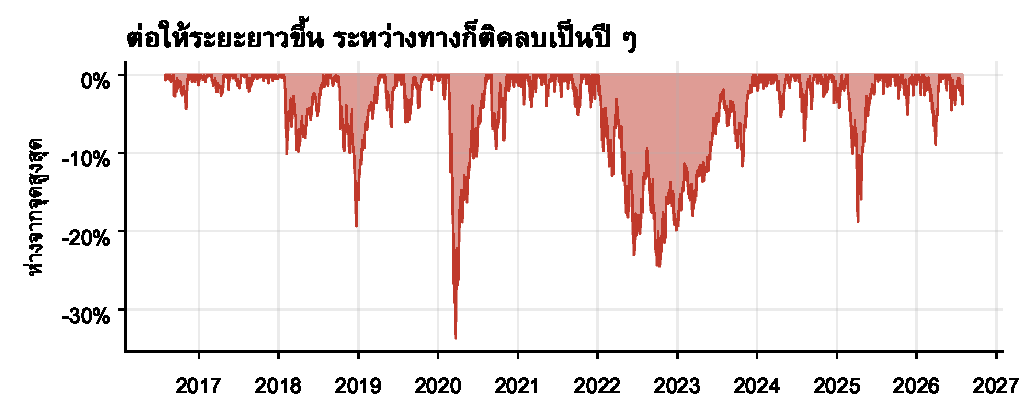
\includegraphics[width=\textwidth]{figures/03-drawdown.pdf}
\caption{\eng{Drawdown} ของ \eng{SPY} --- พื้นที่สีแดงคือช่วงที่ยังไม่กลับไปทำจุดสูงสุดใหม่}
\label{fig:dd}
\end{figure}

\figref{fig:dd} เล่าเรื่องที่กราฟราคาปกติซ่อนไว้ พื้นที่สีแดงกว้างมาก
แปลว่า \textbf{เวลาส่วนใหญ่คุณอยู่ในสภาพ ``ยังไม่กลับไปเท่าจุดสูงสุด''}
ไม่ใช่สภาพ ``กำไรทุกวัน''

\subsection{Sharpe ratio --- ผลตอบแทนต่อความเสี่ยง}

\begin{term}{\eng{Sharpe Ratio}}
\[
\text{Sharpe} = \frac{\text{ผลตอบแทนต่อปี} - \text{ดอกเบี้ยที่ไม่มีความเสี่ยง}}{\text{ความผันผวนต่อปี}}
\]

ตอบคำถามว่า ``ต่อความเสี่ยงหนึ่งหน่วย ได้ผลตอบแทนกลับมาเท่าไหร่''

\begin{center}
\small
\begin{tabular}{ll}
\toprule
ค่า & ความหมายคร่าว ๆ \\
\midrule
ต่ำกว่า 0.5 & ไม่คุ้มความเสี่ยง \\
0.5 -- 1.0 & พอใช้ --- ตลาดหุ้นทั่วไปอยู่แถวนี้ \\
1.0 -- 2.0 & ดี \\
เกิน 2.0 & ดีมาก --- \textbf{และควรสงสัยว่าคำนวณผิดหรือเปล่า} \\
\bottomrule
\end{tabular}
\end{center}

\eng{SPY} 10 ปีที่ผ่านมาได้ \textbf{0.87} ซึ่งถือว่าเป็นช่วงที่ดีผิดปกติของตลาด
\end{term}

\begin{trap}{ทำไม \eng{Sharpe} สูง ๆ ถึงน่าสงสัย}
เวลาเห็นกลยุทธ์ที่อ้าง \eng{Sharpe} เกิน 3 ในผลทดสอบย้อนหลัง
คำอธิบายที่เป็นไปได้มากที่สุดไม่ใช่ ``เจอขุมทรัพย์''
แต่คือ \textbf{มีข้อมูลอนาคตรั่วเข้าไปในการทดสอบ}

บทที่ 7 จะอธิบายว่ารั่วได้อย่างไรบ้าง --- และมันรั่วง่ายกว่าที่คิดมาก
\end{trap}

\subsection{เกณฑ์เปรียบเทียบ อัลฟา และเบตา}

\begin{term}{\eng{Benchmark}, \eng{Alpha}, \eng{Beta}}
\textbf{\eng{Benchmark}} --- เส้นเปรียบเทียบ ถ้ากลยุทธ์คุณทำได้ 12\% ต่อปี
ฟังดูดี แต่ถ้าซื้อ \eng{SPY} เฉย ๆ ได้ 15\% แปลว่าคุณ \emph{แพ้} การนั่งเฉย ๆ

\textbf{\eng{Beta}} --- เคลื่อนไหวตามตลาดแค่ไหน ($\beta = 1$ คือขยับเท่าตลาด,
$\beta = 2$ คือขยับแรงเป็นสองเท่า)

\textbf{\eng{Alpha}} --- ผลตอบแทนส่วนเกินที่\emph{ไม่ได้}มาจากการรับความเสี่ยงตลาด
นี่คือสิ่งที่ทุกคนตามหา และเป็นสิ่งที่หายากที่สุด
\end{term}

\begin{keypoint}
\textbf{ความเข้าใจผิดที่พบบ่อยที่สุด:} ทำกำไรได้ $\neq$ เก่ง

ถ้าตลาดขึ้น 20\% แล้วคุณได้ 15\% คุณไม่ได้เก่ง คุณแค่อยู่ในตลาดที่กำลังขึ้น
และยังทำได้แย่กว่าการไม่ทำอะไรเลย

\textbf{ทุกตัวเลขต้องเทียบกับเกณฑ์เสมอ} --- นี่คือเหตุผลที่โปรเจกต์นี้
รัน 3 กลยุทธ์พื้นฐานคู่ขนานไปตลอดตั้งแต่วันแรก
\end{keypoint}

\subsection{ซื้อ ขายชอร์ต และสภาพคล่อง}

\begin{term}{\eng{Long} และ \eng{Short}}
\textbf{\eng{Long}} --- ซื้อไว้ก่อน หวังว่าราคาจะขึ้น (สิ่งที่คนทั่วไปทำ)

\textbf{\eng{Short}} --- \emph{ยืม}หุ้นมาขายก่อน แล้วค่อยซื้อคืนทีหลัง
กำไรเมื่อราคาลง

การขายชอร์ตสำคัญกับงาน \eng{quant} มาก เพราะมันทำให้เราทำกำไรจาก
``หุ้นตัวนี้แย่กว่าตัวนั้น'' ได้ โดยไม่ต้องเดาว่าตลาดรวมจะขึ้นหรือลง
\end{term}

\begin{term}{สภาพคล่อง (\eng{Liquidity})}
ซื้อขายได้มากแค่ไหนโดยไม่ทำให้ราคาขยับ

หุ้นใหญ่อย่าง \eng{AAPL} ซื้อ 10 ล้านบาทแทบไม่กระเทือนราคา
แต่หุ้นเล็กอาจขยับ 5\% ทันที --- กลยุทธ์ที่ดูดีในกระดาษหลายอันใช้จริงไม่ได้
เพราะสมมติว่าซื้อขายได้ไม่จำกัด
\end{term}

% ═══════════════════════════════════════════════════════════════════════════
\section{ความจริงที่ขัดกับสัญชาตญาณ}
\markboth{ความจริงที่ขัดกับสัญชาตญาณ}{}

บทนี้รวมสิ่งที่ทำให้การลงทุนยากกว่าที่เห็น ทุกข้อมีกราฟจากข้อมูลจริงประกอบ

\subsection{ผลตอบแทนไม่ได้กระจายแบบระฆังคว่ำ}

\begin{figure}[htbp]
\centering
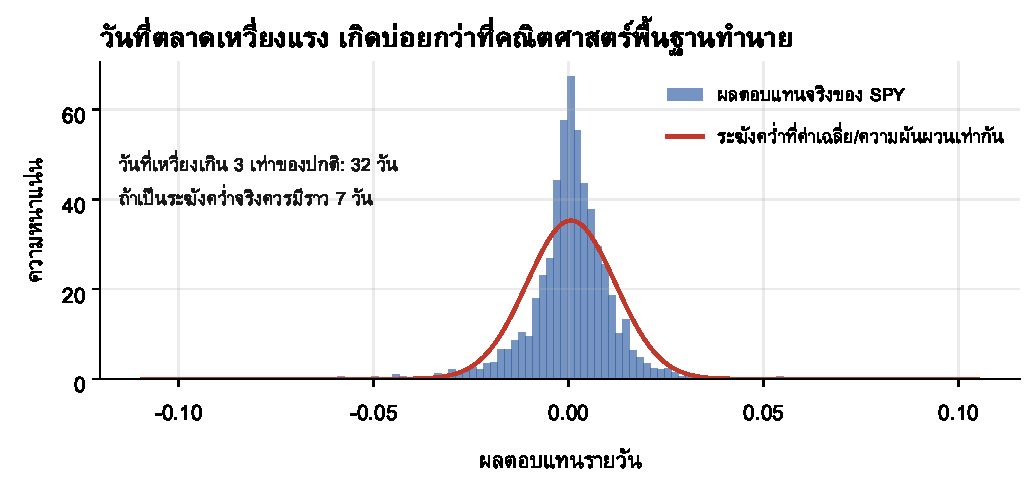
\includegraphics[width=\textwidth]{figures/02-return-distribution.pdf}
\caption{การกระจายของผลตอบแทนรายวันจริง เทียบกับระฆังคว่ำที่มีค่าเฉลี่ยและความผันผวนเท่ากัน}
\label{fig:dist}
\end{figure}

วิชาสถิติพื้นฐานสอนว่าข้อมูลธรรมชาติมักกระจายแบบ ``ระฆังคว่ำ''
และเครื่องมือทางการเงินจำนวนมากก็สร้างบนสมมติฐานนี้

\figref{fig:dist} แสดงว่ามันไม่จริง สังเกตว่าแท่งข้อมูลจริงตรงกลางสูงกว่าเส้นแดง
(วันปกติ ๆ ที่ไม่มีอะไรเกิดขึ้น มีมากกว่าที่ทฤษฎีบอก)
และที่สำคัญกว่าคือ \textbf{ตรงปลายทั้งสองข้าง}

ในข้อมูลจริง 10 ปี มีวันที่ตลาดเหวี่ยงเกิน 3 เท่าของความผันผวนปกติถึง
\textbf{32 วัน} ทั้งที่ถ้าเป็นระฆังคว่ำจริง ควรมีแค่ประมาณ \textbf{7 วัน}

\begin{keypoint}
\textbf{แปลว่า:} เหตุการณ์ ``ที่แทบเป็นไปไม่ได้'' เกิดบ่อยกว่าที่โมเดลคาดไว้ประมาณ 5 เท่า

โมเดลความเสี่ยงที่ใช้ระฆังคว่ำจึงประเมินความเสี่ยงต่ำเกินจริงเสมอ
และนั่นคือสาเหตุที่กองทุนใหญ่ ๆ เจ๊งกันมาแล้วหลายครั้ง
\end{keypoint}

\subsection{ความผันผวนมาเป็นกลุ่ม}

\begin{figure}[htbp]
\centering
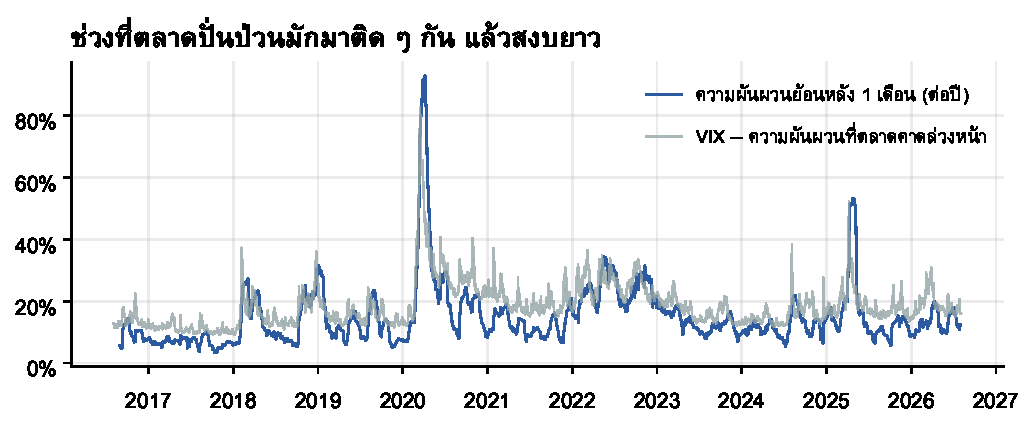
\includegraphics[width=\textwidth]{figures/04-volatility-clustering.pdf}
\caption{ความผันผวนย้อนหลัง 1 เดือน เทียบกับ \eng{VIX} ซึ่งเป็นความผันผวนที่ตลาดคาดล่วงหน้า}
\label{fig:vol}
\end{figure}

ความเสี่ยงไม่ได้กระจายสม่ำเสมอตลอดเวลา แต่มาเป็นก้อน ---
ช่วงสงบยาวหลายเดือน แล้วปั่นป่วนติด ๆ กันหลายสัปดาห์

ข้อดีคือ \textbf{สิ่งนี้พอทำนายได้} ถ้าเมื่อวานเหวี่ยงแรง วันนี้ก็มีแนวโน้มเหวี่ยงแรง
นี่เป็นหนึ่งในไม่กี่อย่างในตลาดที่คาดการณ์ได้จริง และเป็นฐานของโมเดลความเสี่ยงสมัยใหม่

\begin{term}{\eng{VIX} --- ``ดัชนีความกลัว''}
ตัวเลขที่คำนวณจากราคาออปชัน สะท้อนว่า \textbf{ตลาดคาดว่า} อีก 30 วันข้างหน้า
จะผันผวนแค่ไหน

ต่างจากความผันผวนย้อนหลังตรงที่มันมองไปข้างหน้า
โปรเจกต์นี้เก็บ \eng{VIX} ไว้ใช้แบ่ง ``ช่วงสถานการณ์'' ของตลาด
\end{term}

\subsection{พลาดไม่กี่วัน เสียเกือบหมด}

จากข้อมูลจริง 10 ปีของ \eng{SPY}

\begin{center}
\small
\begin{tabular}{lr}
\toprule
จำนวนวันทำการทั้งหมด & 2,514 วัน \\
วันที่ผลตอบแทนเป็นบวก & 55.4\% \\
\midrule
\textbf{ถ้าพลาดแค่ 10 วันที่ดีที่สุด} & \textbf{ผลตอบแทนหายไป 66\%} \\
\bottomrule
\end{tabular}
\end{center}

สิบวัน จากสองพันห้าร้อยวัน คิดเป็น 0.4\% ของเวลาทั้งหมด
แต่มันคือผลตอบแทนสองในสามของทศวรรษ

\begin{trap}{ทำไมการ ``เข้าออกตามจังหวะ'' ถึงอันตราย}
วันที่ดีที่สุดมัก\textbf{เกาะติดกับวันที่แย่ที่สุด} --- ตลาดเด้งแรงที่สุด
ในช่วงที่เพิ่งตกหนัก

คนที่ขายหนีตอนตกหนัก จึงมักไม่อยู่ในตลาดตอนเด้ง
การพยายามหลบวันแย่จึงมักทำให้พลาดวันดีไปด้วย และจบลงแย่กว่าการนั่งเฉย ๆ
\end{trap}

\subsection{ต้นทุนที่มองไม่เห็น}

มือใหม่มักคิดถึงแค่ค่าคอมมิชชัน แต่ต้นทุนจริงมีสามชั้น

\begin{enumerate}
\item \textbf{ค่าคอมมิชชัน} --- ปัจจุบันหลายโบรกเกอร์ในสหรัฐฯ คิด \$0
\item \textbf{ส่วนต่างราคาเสนอซื้อ--ขาย} --- จ่ายทุกครั้งที่ซื้อและขาย
\item \textbf{\eng{Slippage}} --- ราคาที่ได้จริงแย่กว่าราคาที่เห็นตอนกดสั่ง
\end{enumerate}

\begin{trap}{เลขที่ฆ่ากลยุทธ์ส่วนใหญ่}
สมมติต้นทุนรวมแค่ 0.1\% ต่อการซื้อขายหนึ่งรอบ ฟังดูน้อยมาก

แต่ถ้ากลยุทธ์ปรับพอร์ตทุกวัน $= 252$ รอบต่อปี
$\rightarrow$ \textbf{ต้นทุน 25\% ต่อปี}

กลยุทธ์ต้องทำกำไรเกิน 25\% ต่อปีก่อน ถึงจะเริ่มมีกำไรจริง

\textbf{นี่คือเหตุผลที่ผลทดสอบย้อนหลังที่ไม่หักต้นทุน แทบไม่มีความหมายเลย}
\end{trap}

\subsection{สรุปบทนี้}

\begin{keypoint}
\begin{enumerate}
\item เหตุการณ์สุดขั้วเกิดบ่อยกว่าที่ทฤษฎีบอกราว 5 เท่า
\item ความเสี่ยงมาเป็นกลุ่ม --- ซึ่งพอทำนายได้ และเป็นโอกาส
\item ผลตอบแทนกระจุกอยู่ในไม่กี่วัน การหลบตลาดจึงเสี่ยงกว่าที่คิด
\item ต้นทุนการซื้อขายกินกำไรเร็วกว่าที่ใคร ๆ ประเมิน
\end{enumerate}

ทั้งสี่ข้อรวมกันอธิบายว่า ทำไมนักลงทุนส่วนใหญ่ถึงแพ้การซื้อกองทุนดัชนีแล้วนั่งเฉย ๆ
\end{keypoint}

% ═══════════════════════════════════════════════════════════════════════════
\section{Quant คืออะไร}
\markboth{Quant คืออะไร}{}

\subsection{นิยามที่ใช้ได้จริง}

\begin{term}{การลงทุนเชิงปริมาณ (\eng{Quantitative Investing})}
การตัดสินใจลงทุนด้วย \textbf{กฎที่เขียนเป็นสูตรได้ ทดสอบซ้ำได้ และไม่ขึ้นกับอารมณ์}
แทนการใช้วิจารณญาณรายกรณี

ความต่างที่แท้จริงไม่ใช่ ``ใช้คอมพิวเตอร์'' แต่คือ \textbf{ทุกการตัดสินใจต้องอธิบายได้
ว่ามาจากกฎข้อไหน และกฎข้อนั้นเคยถูกทดสอบแล้วว่าใช้ได้จริงไหม}
\end{term}

นักลงทุนแบบดั้งเดิมอาจบอกว่า ``ผมชอบบริษัทนี้ ผู้บริหารเก่ง''
ซึ่งอาจถูกก็ได้ แต่ทดสอบไม่ได้ ทำซ้ำไม่ได้ และไม่รู้ว่าเคยถูกกี่ครั้งจากทั้งหมดกี่ครั้ง

นักลงทุนเชิงปริมาณจะบอกว่า ``ซื้อหุ้น 20\% บนที่มีอัตราส่วนกำไรต่อราคาสูงสุด
ปรับพอร์ตทุกเดือน'' ซึ่ง \textbf{ทดสอบย้อนหลัง 30 ปีได้ทันที}

\subsection{Factor --- หัวใจของทุกอย่าง}

\begin{term}{\eng{Factor} (ปัจจัย)}
ตัวเลขที่คำนวณจากข้อมูลที่มีอยู่ ณ วันนี้ แล้ว\textbf{หวังว่า}จะบอกอะไรบางอย่าง
เกี่ยวกับผลตอบแทนในอนาคตได้

ตัวอย่าง \eng{factor} คลาสสิกที่มีงานวิจัยรองรับหลายสิบปี

\begin{center}
\small
\begin{tabular}{lll}
\toprule
ชื่อ & คำนวณจาก & สมมติฐาน \\
\midrule
\eng{Momentum} & ผลตอบแทน 12 เดือนที่ผ่านมา & ตัวที่ขึ้นดี มักขึ้นต่ออีกพัก \\
\eng{Value} & กำไร $\div$ ราคา & ของถูกให้ผลตอบแทนดีกว่าระยะยาว \\
\eng{Size} & มูลค่าตลาด & บริษัทเล็กเสี่ยงกว่า จึงได้ผลตอบแทนสูงกว่า \\
\eng{Low Volatility} & ความผันผวนย้อนหลัง & ตัวที่นิ่งกว่ากลับให้ผลดีกว่า \\
\bottomrule
\end{tabular}
\end{center}
\end{term}

\subsection{Momentum --- ดูของจริง}

\begin{figure}[htbp]
\centering
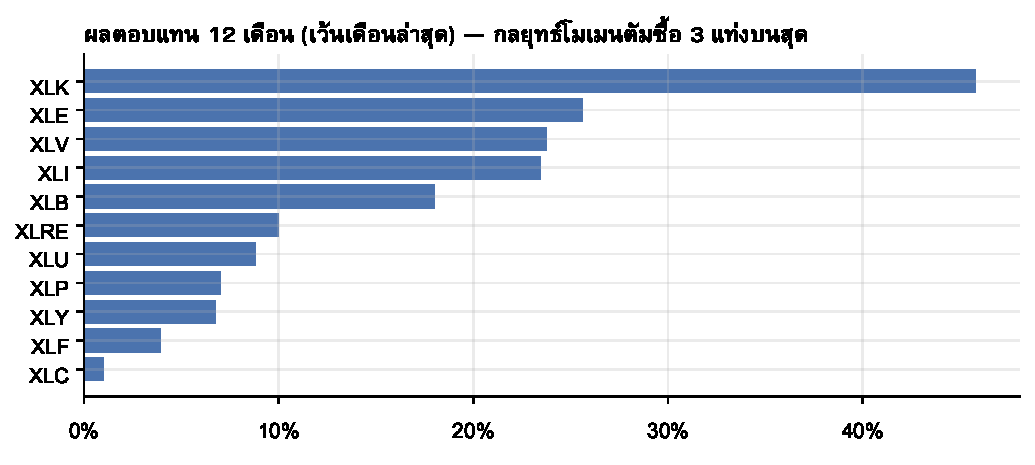
\includegraphics[width=\textwidth]{figures/07-momentum.pdf}
\caption{ผลตอบแทน 12 เดือนของแต่ละกลุ่มธุรกิจ (เว้นเดือนล่าสุด) --- กลยุทธ์โมเมนตัมจะซื้อ 3 แท่งบนสุด}
\label{fig:mom}
\end{figure}

\figref{fig:mom} คือ \eng{factor} ตัวจริงที่ทำงานอยู่ในโปรเจกต์นี้
ทุกเดือนระบบจะจัดอันดับกลุ่มธุรกิจทั้ง 11 กลุ่มตามผลตอบแทนย้อนหลัง
แล้วซื้อ 3 กลุ่มที่ดีที่สุด

\begin{term}{ทำไมต้อง ``เว้นเดือนล่าสุด''}
สูตรมาตรฐานเรียกว่า \eng{12-1 momentum} --- ดูผลตอบแทน 12 เดือน
แต่\textbf{ตัดเดือนล่าสุดทิ้ง}

เหตุผล: ในระยะสั้นมาก (1 เดือน) ราคามีแนวโน้ม \emph{กลับทิศ} ไม่ใช่ไปต่อ
ถ้าไม่ตัดออก \eng{factor} สองตัวที่ขัดกันจะหักล้างกันเอง

รายละเอียดเล็ก ๆ แบบนี้คือความต่างระหว่างกลยุทธ์ที่ใช้ได้กับใช้ไม่ได้
\end{term}

\subsection{จัดอันดับข้ามหุ้น กับ ดูตัวเดียวข้ามเวลา}

นี่คือแนวคิดที่สำคัญที่สุดในบทนี้ และเป็นตัวกำหนดทิศทางของโปรเจกต์ทั้งหมด

\begin{term}{\eng{Cross-sectional} เทียบกับ \eng{Time-series}}
\textbf{\eng{Cross-sectional}} --- ``วันนี้ในบรรดาหุ้น 500 ตัว ตัวไหนน่าซื้อที่สุด''

ซื้อกลุ่มที่คะแนนสูงสุด ขายชอร์ตกลุ่มที่ต่ำสุด กำไรจาก\emph{ความต่าง}
ไม่ต้องเดาว่าตลาดรวมจะขึ้นหรือลง

\vspace{0.5em}
\textbf{\eng{Time-series}} --- ``หุ้นตัวนี้ ตอนนี้ควรถือหรือไม่ถือ''

ตัดสินจากประวัติของตัวมันเอง
\end{term}

ความต่างสำคัญตรงที่ \textbf{จำนวนตัวอย่างที่ใช้ทดสอบได้}

\begin{center}
\small
\begin{tabular}{lrl}
\toprule
วิธี & ตัวอย่างต่อ 1 ปี & หมายเหตุ \\
\midrule
\eng{Time-series} หุ้น 1 ตัว & 252 & ต้องรอหลายปีกว่าจะสรุปอะไรได้ \\
\eng{Cross-sectional} 500 ตัว & 126{,}000 & สรุปได้เร็วกว่ามาก \\
\bottomrule
\end{tabular}
\end{center}

\begin{trap}{ข้อจำกัดที่โปรเจกต์นี้เจอโดยตรง}
เดิมโปรเจกต์ติดตามหุ้นแค่ 8 ตัว ซึ่ง\textbf{จัดอันดับไม่ได้}
--- จะซื้อกลุ่มบนขายกลุ่มล่างจาก 8 ตัว แปลว่ากลุ่มละ 2--3 ตัว ซึ่งสุ่มเกินไป

นี่คือเหตุผลที่ล่าสุดเราขยายเป็น 24 ตัว ครอบคลุมทั้ง 11 กลุ่มธุรกิจ
รายละเอียดอยู่ในบทที่ 8
\end{trap}

\subsection{หุ้นเคลื่อนไหวไปด้วยกันแค่ไหน}

\begin{figure}[htbp]
\centering
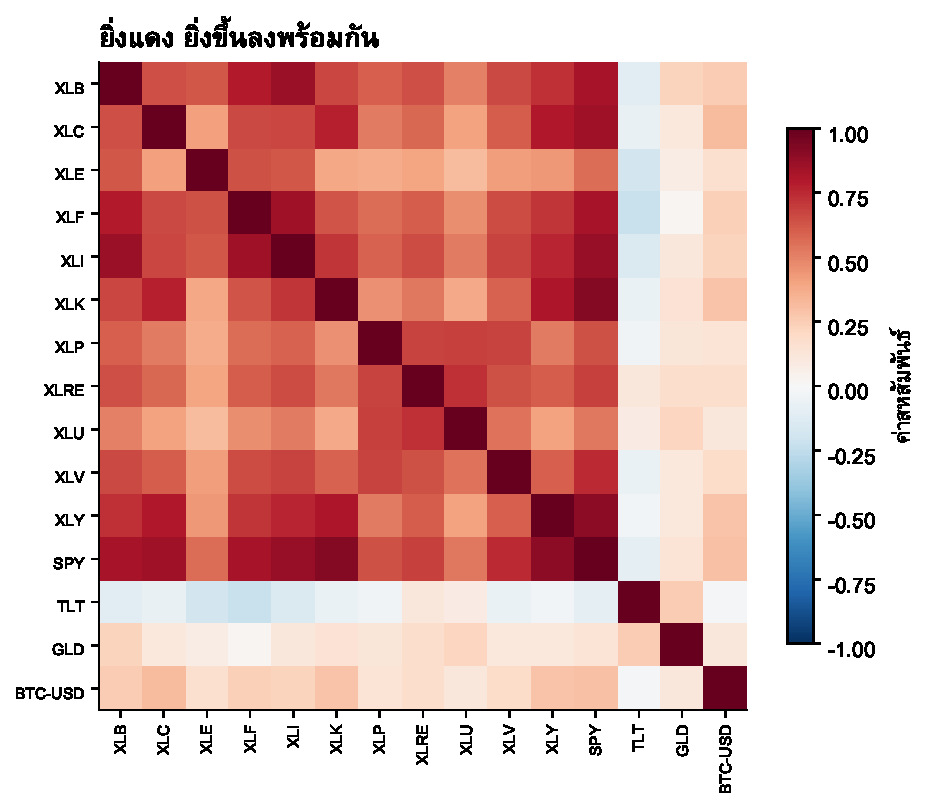
\includegraphics[width=0.86\textwidth]{figures/06-correlation.pdf}
\caption{ค่าสหสัมพันธ์ของผลตอบแทนรายวัน --- ยิ่งแดงยิ่งขึ้นลงพร้อมกัน}
\label{fig:corr}
\end{figure}

\figref{fig:corr} บอกอะไรที่สำคัญมากเรื่องการกระจายความเสี่ยง

กลุ่มธุรกิจต่าง ๆ (\eng{XL}\ldots) เป็นสีแดงเข้มเกือบหมด แปลว่า
\textbf{การซื้อหุ้นหลายกลุ่มไม่ได้กระจายความเสี่ยงอย่างที่คิด} ---
เวลาตลาดตก มันตกพร้อมกัน

ส่วน \eng{TLT} (พันธบัตร) และ \eng{GLD} (ทองคำ) มีสีอ่อนหรือออกไปทางน้ำเงิน
นั่นคือการกระจายความเสี่ยงที่แท้จริง

\begin{keypoint}
\textbf{การกระจายความเสี่ยงที่แท้จริงมาจากการถือของที่เคลื่อนไหวคนละทาง}
ไม่ใช่การถือของหลายอย่างที่เคลื่อนไหวเหมือนกัน

นี่คือเหตุผลที่กลยุทธ์ ``หุ้น 60\% พันธบัตร 40\%'' ยังคงเป็นเกณฑ์มาตรฐาน
มาหลายสิบปี ทั้งที่ดูเรียบง่ายมาก
\end{keypoint}

\subsection{วัดว่า Factor ดีแค่ไหน}

\begin{term}{\eng{Information Coefficient} (IC)}
ค่าสหสัมพันธ์ระหว่าง \emph{คะแนนที่ \eng{factor} ให้วันนี้} กับ
\emph{ผลตอบแทนที่เกิดขึ้นจริงในวันถัดไป}

\begin{center}
\small
\begin{tabular}{ll}
\toprule
\eng{IC} & ความหมาย \\
\midrule
0.00 & ไม่มีข้อมูลเลย เท่ากับเดาสุ่ม \\
0.02 -- 0.05 & \textbf{ใช้ได้จริงในวงการ} \\
เกิน 0.10 & ดีผิดปกติ --- ควรกลับไปหาว่าข้อมูลอนาคตรั่วตรงไหน \\
\bottomrule
\end{tabular}
\end{center}
\end{term}

ตัวเลขนี้ทำให้มือใหม่ตกใจเสมอ --- \eng{IC} เพียง 0.03 ฟังดูเหมือนแทบไม่มีสัญญาณ
แต่มันคือระดับที่กองทุนระดับโลกใช้ทำกำไรจริง

เหตุผลคือ \eng{factor} ถูกใช้กับหุ้นหลายร้อยตัวพร้อมกันและซ้ำ ๆ ทุกวัน
เหมือนคาสิโนที่ได้เปรียบแค่ 1\% ต่อเกม แต่เล่นเป็นล้านเกม

\begin{keypoint}
งานวิจัย \eng{RD-Agent(Q)} ที่โปรเจกต์นี้ใช้เป็นแนวทาง รายงาน \eng{IC} ที่ \textbf{0.0532}
--- ซึ่งอยู่ในระดับ ``ดีมาก'' ตามมาตรฐานวงการ ไม่ใช่ ``น่าสงสัย''
\end{keypoint}

% ═══════════════════════════════════════════════════════════════════════════
\section{กับดักที่ทำให้ผลทดสอบโกหก}
\markboth{กับดักที่ทำให้ผลทดสอบโกหก}{}

\begin{term}{\eng{Backtest} --- การทดสอบย้อนหลัง}
เอากฎที่คิดไว้ ไปลองกับข้อมูลในอดีต แล้วดูว่าถ้าทำแบบนี้จริงจะได้เท่าไหร่
\end{term}

ฟังดูตรงไปตรงมา แต่ \textbf{นี่คือจุดที่งานวิจัยในวงการนี้ผิดพลาดกันมากที่สุด}
บทนี้อธิบายว่าผิดได้อย่างไรบ้าง

\subsection{กับดักที่ 1 --- ปรับจนพอดีเกินไป}

\begin{trap}{\eng{Overfitting}}
ถ้าคุณลองกฎ 1,000 แบบกับข้อมูลชุดเดียวกัน จะมีสัก 50 แบบที่ได้ผลดีมาก
\textbf{ด้วยความบังเอิญล้วน ๆ}

พอเลือกอันที่ดีที่สุดมาอวด มันจึงดูดีเกินจริงเสมอ และพอใช้เงินจริงก็พัง

\textbf{ยิ่งลองเยอะ ยิ่งต้องสงสัยผลลัพธ์มากขึ้น} ไม่ใช่น้อยลง
\end{trap}

วิธีป้องกันที่ได้ผลจริงมีอยู่ทางเดียวคือ \textbf{เขียนสมมติฐานลงกระดาษก่อนดูข้อมูล}
แล้วทดสอบครั้งเดียว --- โปรเจกต์นี้มีระบบ \code{finbg hypo} ไว้ทำเรื่องนี้โดยเฉพาะ

\subsection{กับดักที่ 2 --- ใช้ข้อมูลที่ตอนนั้นยังไม่มี}

\begin{trap}{\eng{Look-ahead Bias}}
ตัวอย่างที่เกิดบ่อยที่สุด: ใช้งบการเงินไตรมาสที่ 1 ตัดสินใจซื้อขายวันที่
31 มีนาคม ทั้งที่งบนั้น \textbf{ประกาศจริงวันที่ 25 เมษายน}

ผลทดสอบจะสวยงามมาก เพราะคุณกำลังซื้อขายด้วยข้อมูลที่ยังไม่มีใครรู้
\end{trap}

\begin{term}{\eng{Point-in-Time} (PIT) --- วิธีป้องกัน}
ทุกข้อมูลต้องเก็บ \textbf{สองวันที่}

\begin{itemize}
\item \code{event\_date} --- วันที่เหตุการณ์เกิดจริง
\item \code{knowledge\_date} --- วันที่เรา\emph{รู้}เรื่องนี้
\end{itemize}

แล้วเวลาทดสอบ ให้ใช้เฉพาะข้อมูลที่ \code{knowledge\_date} มาก่อนวันตัดสินใจ

โปรเจกต์นี้บังคับให้ทุกไฟล์ที่บันทึกต้องมีช่อง \code{fetched\_at}
และ \textbf{ห้ามเขียนทับไฟล์เดิมเด็ดขาด} --- ทุกครั้งที่ดึงข้อมูลจะได้ไฟล์ใหม่
พร้อมเวลาที่ดึงของตัวเอง
\end{term}

\subsection{กับดักที่ 3 --- นับเฉพาะผู้รอดชีวิต}

\begin{trap}{\eng{Survivorship Bias}}
ถ้าคุณทดสอบกับ ``หุ้นที่อยู่ใน \eng{S\&P 500} วันนี้'' ย้อนหลัง 20 ปี
คุณกำลังทดสอบกับ \textbf{บริษัทที่รอดมาได้เท่านั้น}

บริษัทที่ล้มละลายหายไประหว่างทางไม่อยู่ในข้อมูล ผลตอบแทนจึงสูงเกินจริงเสมอ
ประมาณ 1--2\% ต่อปี ซึ่งมากพอจะเปลี่ยนกลยุทธ์ที่ขาดทุนให้ดูเหมือนกำไร
\end{trap}

\subsection{กับดักที่ 4 --- รู้อนาคตแล้วมาตัดสินอดีต}

กับดักนี้เกี่ยวข้องกับโปรเจกต์นี้โดยตรงที่สุด

\begin{trap}{\eng{Hindsight Bias} --- อคติเพราะรู้ผลแล้ว}
สมมติวันที่ 30 ก.ค. \eng{Apple} ยื่นเอกสาร \eng{8-K} ต่อ ก.ล.ต. สหรัฐฯ
พาดหัวบอกแค่ว่า ``มีการยื่นเอกสาร'' ไม่ได้บอกว่าดีหรือร้าย

ต่อมาวันที่ 3 ส.ค. ข่าวออกว่า \eng{Apple} มูลค่าหายไป \$500{,}000 ล้าน

\vspace{0.5em}
ทีนี้ถ้าเรามาติดป้ายข่าววันที่ 30 ก.ค. \emph{ในวันที่ 5 ส.ค.}
เราจะอดใจไม่ไหวที่จะติดว่า ``เชิงลบ'' --- ทั้งที่ ณ วันนั้นไม่มีใครรู้

ผลคือคลังข้อมูลจะดู ``แม่นยำอย่างน่าทึ่ง'' แต่เป็นความแม่นที่เกิดจากการรู้อนาคต
\textbf{ใช้สอนโมเดลไม่ได้เลย เพราะตอนใช้งานจริงจะไม่มีข้อมูลแบบนั้น}
\end{trap}

\begin{keypoint}
\textbf{ทางแก้ในโปรเจกต์นี้} มีสามชั้น

\begin{enumerate}
\item ติดป้ายข่าว \textbf{ให้เร็วที่สุดหลังข่าวออก} --- ระบบอัตโนมัติทำงานทุกวัน 06:30 น.
      ห่างจากตอนเก็บข่าวแค่ 30 นาที
\item บันทึกช่อง \code{days\_after\_publish} ไว้ทุกรายการ
      --- ทำให้ย้อนกลับไปตรวจได้ว่ารายการไหนติดป้ายช้าจนน่าสงสัย
\item ระบบเตือนอัตโนมัติเมื่อมีรายการที่ติดป้ายหลังข่าวออกเกิน 7 วัน
\end{enumerate}

ข้อ 2 สำคัญเป็นพิเศษ เพราะทำให้เรา \textbf{วัดการปนเปื้อนของตัวเองได้}
ซึ่งเป็นสิ่งที่งานวิจัยที่ตีพิมพ์ส่วนใหญ่ทำไม่ได้
\end{keypoint}

\subsection{ทำไมเกณฑ์เปรียบเทียบถึงสำคัญกว่ากลยุทธ์}

\begin{figure}[htbp]
\centering
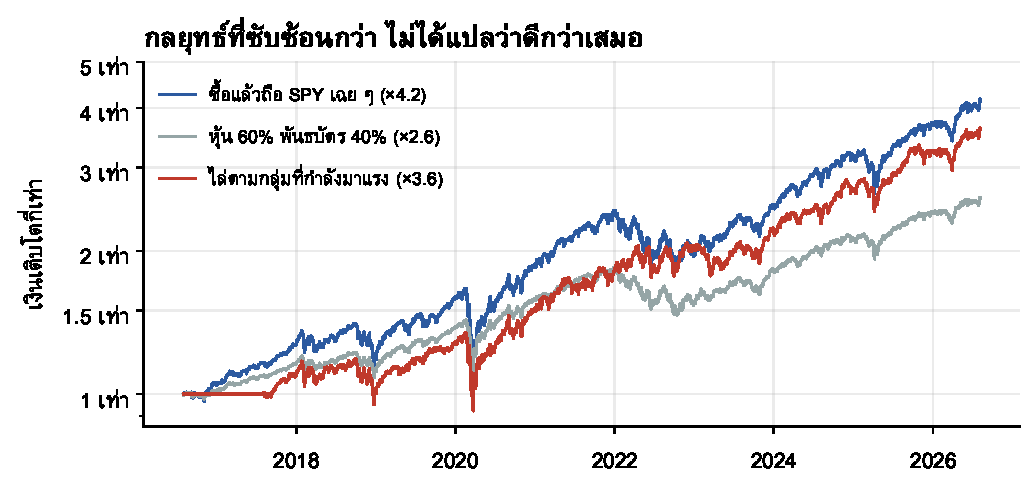
\includegraphics[width=\textwidth]{figures/05-baselines.pdf}
\caption{กลยุทธ์พื้นฐาน 3 แบบที่โปรเจกต์นี้รันคู่ขนานตั้งแต่วันแรก}
\label{fig:base}
\end{figure}

\figref{fig:base} คือเหตุผลที่ต้องมีเกณฑ์เปรียบเทียบ

กลยุทธ์ ``ไล่ตามกลุ่มที่กำลังมาแรง'' ซึ่งซับซ้อนที่สุดในสามอัน
ได้ผลตอบแทน \textbf{3.6 เท่า} ฟังดูดีมาก\ldots จนกระทั่งเห็นว่า
การซื้อ \eng{SPY} แล้วนอนหลับได้ \textbf{4.2 เท่า}

\begin{keypoint}
\textbf{ถ้าไม่มีเส้นเปรียบเทียบ คุณจะไม่มีทางรู้เลยว่ากลยุทธ์ที่อุตส่าห์สร้าง
จริง ๆ แล้วแย่กว่าการไม่ทำอะไร}

นี่คือเหตุผลที่โปรเจกต์นี้สร้างระบบบันทึกผล 3 กลยุทธ์พื้นฐาน
\emph{ก่อน} จะเริ่มสร้างกลยุทธ์ของตัวเอง
\end{keypoint}

% ═══════════════════════════════════════════════════════════════════════════
\section{AI กับการลงทุน --- อะไรได้ผลจริง}
\markboth{AI กับการลงทุน}{}

\subsection{ข้อสรุปที่ขัดกับสิ่งที่ขายกันในตลาด}

เมื่อค้นงานวิจัยล่าสุดอย่างเป็นระบบ จะพบข้อสรุปที่ตรงกันจากหลายกลุ่มวิจัยอิสระ

\begin{keypoint}
\textbf{LLM ล้มเหลว} ในบทบาท \emph{ผู้ตัดสินใจซื้อขาย}

\textbf{LLM ได้ผลดี} ในบทบาท \emph{นักวิจัยที่เขียน factor ออกมาเป็นโค้ด}
\end{keypoint}

\subsection{ทำไมให้ AI เทรดเองถึงไม่ได้ผล}

\begin{trap}{ปัญหาเชิงสถาปัตยกรรม ไม่ใช่แค่ ``ยังไม่เก่งพอ''}
LLM สร้างคำตอบแบบทีละคำโดยมีความสุ่มอยู่ในตัว ผลคือ

\begin{itemize}
\item ถามคำถามเดิม สองครั้ง ได้คำตอบต่างกัน
\item วันนี้บอกให้ซื้อ พรุ่งนี้บอกให้ขาย ทั้งที่ข้อมูลแทบไม่เปลี่ยน
      (เรียกว่า \eng{action flipping})
\item ไม่มีความจำสถานะที่มั่นคงระหว่างการตัดสินใจแต่ละครั้ง
\end{itemize}

งานวิจัย \eng{FINSABER} (2026) ทดสอบกลยุทธ์ที่ขับเคลื่อนด้วย LLM
ในกรอบเวลายาว พบว่า \textbf{แพ้การซื้อแล้วถือเฉย ๆ} และมีรูปแบบความผิดพลาดที่ชัดเจน:
ระมัดระวังเกินไปตอนตลาดขาขึ้น และก้าวร้าวเกินไปตอนตลาดขาลง
\end{trap}

\subsection{ทำไมให้ AI เป็นนักวิจัยถึงได้ผล}

ความต่างอยู่ที่ \textbf{ผลลัพธ์ที่ขอจากมัน}

\begin{center}
\small
\begin{tabular}{lll}
\toprule
 & AI เป็นเทรดเดอร์ & AI เป็นนักวิจัย \\
\midrule
ผลลัพธ์ & ``ซื้อ 100 หุ้น'' & โค้ดที่คำนวณ \eng{factor} \\
ตรวจสอบได้ไหม & ไม่ได้ทันที & \textbf{ได้ --- รันทดสอบย้อนหลังเลย} \\
ถ้าตอบมั่ว & เสียเงินจริง & \textbf{ทดสอบไม่ผ่าน แล้วทิ้ง} \\
ความไม่แน่นอน & เป็นปัญหา & \textbf{เป็นข้อดี --- ได้ไอเดียหลากหลาย} \\
\bottomrule
\end{tabular}
\end{center}

\begin{keypoint}
ประเด็นสำคัญคือ \textbf{มีตัวกรองที่เป็นกลางคั่นอยู่}

AI เสนอไอเดีย $\rightarrow$ ระบบทดสอบย้อนหลังตัดสิน $\rightarrow$ อันที่ไม่ผ่านถูกทิ้ง

AI ไม่ได้แตะเงินโดยตรงเลย มันแค่เสนอสมมติฐานให้ระบบที่เข้มงวดคัดกรอง
\textbf{ความไม่เสถียรที่เป็นจุดอ่อนตอนเทรด กลายเป็นจุดแข็งตอนคิดไอเดีย}
\end{keypoint}

\subsection{หลักฐานที่ชัดที่สุด}

\begin{center}
\small
\begin{tabular}{ll}
\toprule
\multicolumn{2}{l}{\textbf{\eng{RD-Agent(Q)}} --- ตีพิมพ์ใน \eng{NeurIPS} 2025} \\
\midrule
\eng{IC} & 0.0532 (ระดับใช้ได้จริงในวงการ) \\
ผลตอบแทนต่อปี & 14.21\% \\
เทียบกับคลัง \eng{factor} ดั้งเดิม & ผลตอบแทน 2 เท่า ด้วย \eng{factor} น้อยกว่า 70\% \\
ค่าใช้จ่ายทั้งการทดลอง & น้อยกว่า \$10 \\
\bottomrule
\end{tabular}
\end{center}

ตัวเลขสุดท้ายสำคัญที่สุดสำหรับเรา --- งานระดับตีพิมพ์ทำได้ด้วยงบไม่ถึง \$10
แปลว่า \textbf{อุปสรรคไม่ใช่เงิน แต่คือระเบียบวิธีที่ถูกต้อง}

% ═══════════════════════════════════════════════════════════════════════════
\section{โปรเจกต์นี้ทำอะไรอยู่}
\markboth{โปรเจกต์นี้ทำอะไรอยู่}{}

\subsection{เป้าหมายและกลยุทธ์หลัก}

เป้าหมายระยะยาวคือสร้างระบบที่ให้ AI ช่วยค้นหา \eng{factor} ใหม่
แล้วมีระบบทดสอบที่เข้มงวดพอจะบอกได้ว่า \eng{factor} นั้นจริงหรือปลอม

แต่กลยุทธ์ที่ใช้เดินไปถึงจุดนั้นมีจุดสำคัญอยู่ข้อหนึ่ง

\begin{keypoint}
\textbf{งานบางอย่างเร่งไม่ได้ ต้องเริ่มวันนี้ --- งานบางอย่างทำเมื่อไหร่ก็ได้}

\begin{center}
\small
\begin{tabular}{lll}
\toprule
งาน & ย้อนหลังทำได้ไหม & ความเร่งด่วน \\
\midrule
ราคาหุ้นย้อน 10 ปี & ได้ ดึงเมื่อไหร่ก็เหมือนกัน & ไม่เร่ง \\
คำนวณ \eng{factor} จากราคา & ได้ & ไม่เร่ง \\
สรุปงานวิจัย & ได้ & ไม่เร่ง \\
\midrule
\textbf{เก็บข่าวรายวัน} & \textbf{ไม่ได้} & \textbf{เร่งที่สุด} \\
\textbf{ติดป้ายข่าว} & \textbf{ไม่ได้ --- ปนเปื้อนทันที} & \textbf{เร่ง} \\
\textbf{บันทึกคำทำนายล่วงหน้า} & \textbf{ไม่ได้} & \textbf{เร่ง} \\
\bottomrule
\end{tabular}
\end{center}

ข่าวเมื่อวานที่ไม่ได้เก็บ ไม่มีทางเก็บย้อนหลังได้ในสภาพที่สะอาด
ทุกวันที่ผ่านไปโดยไม่เก็บ คือข้อมูลที่หายถาวร
\end{keypoint}

\subsection{ระบบที่ทำงานอยู่จริงตอนนี้}

\begin{center}
\small
\begin{tabular}{lll}
\toprule
เวลา & ระบบ & ทำอะไร \\
\midrule
06:00 น. & \code{daily.sh} & เก็บราคา 28 ตัว, ข่าว 4 แหล่ง, คำนวณผลกลยุทธ์พื้นฐาน \\
06:30 น. & \code{label-auto.sh} & เปิด AI มาอ่านข่าวและติดป้ายอัตโนมัติ \\
อาทิตย์ 07:30 & \code{backup.sh} & สำรองข้อมูลทั้งหมด \\
\bottomrule
\end{tabular}
\end{center}

ทั้งหมดทำงานเองโดยไม่ต้องเปิดหน้าจอทิ้งไว้ ค่าใช้จ่ายราว \$0.5 ต่อวัน

\begin{figure}[htbp]
\centering
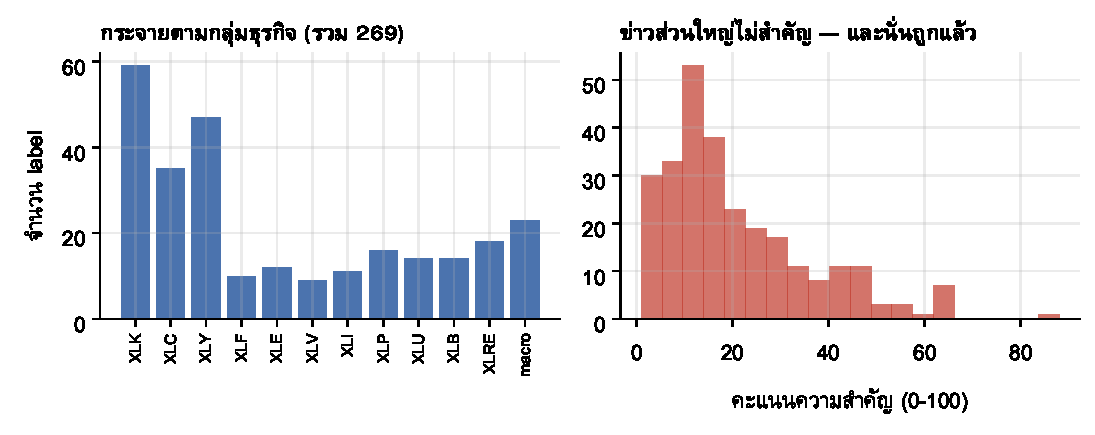
\includegraphics[width=\textwidth]{figures/08-corpus.pdf}
\caption{คลังข่าวที่ติดป้ายแล้ว ณ วันที่ทำเอกสารนี้ --- 269 รายการ}
\label{fig:corpus}
\end{figure}

\subsection{การตัดสินใจออกแบบที่สำคัญ}

\subsubsection{ทำไมต้องกรองข่าวก่อนติดป้าย}

ระบบเก็บข่าวได้วันละ 500--1{,}200 ชิ้น ซึ่งติดป้ายไม่ไหวไม่ว่าจะใช้ AI ตัวไหน
จึงกรองเหลือเฉพาะที่เป็นเอกสารต้นทาง (เช่น เอกสารที่ยื่นต่อ ก.ล.ต.)
หรือยืนยันได้ว่าเกี่ยวกับหุ้นในรายชื่อที่ติดตาม

สิ่งที่ตัดออกส่วนใหญ่เป็นบทความชวนคลิก ซึ่งได้คะแนนความสำคัญต่ำอยู่แล้ว
\textbf{การกรองจึงทำให้คลังดีขึ้น ไม่ใช่แย่ลง}

\subsubsection{ทำไมต้องมีโควตาต่อกลุ่มธุรกิจ}

\begin{trap}{ปัญหาที่วัดได้จากข้อมูลจริง}
ในคลัง 105 รายการแรก หุ้น \eng{AMZN}, \eng{MSFT}, \eng{AAPL}, \eng{META}
กินไป \textbf{67 จาก 98 ครั้ง} ที่มีการอ้างถึงหุ้น

คลังแบบนี้ไม่ใช่ ``ภาพรวมตลาด'' แต่เป็น ``ข่าวบริษัทเทคโนโลยียักษ์ใหญ่''
ซึ่งใช้ทำงานจัดอันดับข้ามหุ้นไม่ได้เลย
\end{trap}

ทางแก้คือกำหนดเพดานว่าแต่ละกลุ่มธุรกิจ ในแต่ละวัน จะติดป้ายได้ไม่เกิน 6 ชิ้น
ผลคือได้คลังที่สมดุลกว่า และควบคุมค่าใช้จ่ายไปพร้อมกัน

\begin{keypoint}
\textbf{6 ชิ้นจาก 12 กลุ่ม มีค่ามากกว่า 72 ชิ้นที่มาจาก 3 กลุ่ม}
ทั้งที่จำนวนเท่ากัน --- เพราะโมเดลจัดอันดับต้องการความสมดุล ไม่ใช่ปริมาณ
\end{keypoint}

\subsubsection{บทเรียนจากบั๊กที่เจอจริง}

\begin{trap}{จับชื่อย่อหุ้นด้วยการค้นข้อความธรรมดา}
โค้ดเดิมตรวจว่าพาดหัวมีคำว่า \eng{META} ไหม ด้วยการค้นข้อความตรง ๆ

ผลคือข่าว ``\eng{This Overlooked \textbf{Metal}s Stock\ldots}'' ถูกติดป้ายว่าเป็นข่าว
\eng{Meta} เพราะคำว่า \eng{Metal} มีตัวอักษร \eng{META} อยู่ข้างใน

ยิ่งอันตรายเมื่อเพิ่มหุ้นใหม่ เพราะ \eng{CAT} (\eng{Caterpillar}) ตรงกับคำว่า ``แมว''
และ \eng{KO} (\eng{Coca-Cola}) ตรงกับคำว่า ``น็อกเอาต์''
\end{trap}

ทางแก้มีสองชั้น

\begin{enumerate}
\item ตรวจแบบ \textbf{ขอบเขตคำ} ไม่ใช่ข้อความย่อย
\item ชื่อย่อที่บังเอิญเป็นคำปกติ (\eng{CAT}, \eng{KO}, \eng{GE}, \eng{LIN}, \eng{PG},
      \eng{AMT}, \eng{NEE}) \textbf{ห้ามจับจากชื่อย่อเลย} ให้จับจากชื่อบริษัทเต็มแทน
\end{enumerate}

แต่การแก้ครั้งแรกสร้างปัญหาใหม่ทันที --- ตัวตรวจขอบเขตคำมาตรฐาน
นับอักษรจีนเป็นตัวอักษรด้วย ทำให้พาดหัวภาษาจีนที่มีคำว่า \eng{Amazon}
อยู่กลางประโยคจับไม่ได้เลย ซึ่งเป็นปัญหาใหญ่เพราะแหล่งข่าวหนึ่งส่งข่าวหลายภาษามา

ทางแก้สุดท้ายคือนิยามขอบเขตด้วย \textbf{ตัวอักษรละตินและตัวเลขเท่านั้น}

\begin{keypoint}
\textbf{บทเรียนที่ใช้ได้ทั่วไป:} การทดสอบไม่ใช่พิธีกรรม

บั๊กทั้งสามตัวในโปรเจกต์นี้ (ข่าวซ้ำ, ติดป้ายผิดตัว, เขียนไฟล์ไม่ได้)
ถูกเจอเพราะ\textbf{ลองรันจริงแล้วตรวจผลทีละบรรทัด} ไม่ใช่เพราะอ่านโค้ดแล้วนึกออก
\end{keypoint}

% ═══════════════════════════════════════════════════════════════════════════
\section{แผนงานข้างหน้า}
\markboth{แผนงานข้างหน้า}{}

\subsection{ภาพรวม 18 เดือน}

\begin{center}
\small
\begin{tabular}{cllc}
\toprule
เฟส & ช่วง & เป้าหมาย & ประตูผ่าน \\
\midrule
--- & ส.ค. 2026 & วิจัยเครื่องมือและวางแผน & \textbf{เสร็จแล้ว} \\
0 & เดือน 1--2 & ระบบทดสอบและชั้นข้อมูล & ระบบปฏิเสธ \eng{factor} ปลอมได้ \\
1 & เดือน 3--5 & \eng{Quant} คลาสสิก & ทำซ้ำผลงานมาตรฐานได้ \\
2 & เดือน 6--9 & AI เป็นนักวิจัย & ทำซ้ำ \eng{RD-Agent(Q)} ได้ \\
3 & เดือน 10--14 & งานวิจัยต้นฉบับ & \eng{factor} ที่เพิ่มค่าเหนือเกณฑ์ \\
4 & เดือน 15--18 & ทดลองด้วยเงินจริงน้อย ๆ & ผลจริงตรงกับผลทดสอบ \\
\bottomrule
\end{tabular}
\end{center}

\subsection{คำถามวิจัยที่คลังข่าวจะตอบ}

คลังข่าวที่กำลังสะสมอยู่มีไว้ตอบคำถามเดียว

\begin{keypoint}
\textbf{``ถ้าเพิ่มข้อมูลข่าวเข้าไปในโมเดล \eng{quant} ที่มีอยู่ มันดีขึ้นไหม''}

สังเกตว่าไม่ใช่คำถามว่า ``ข่าวทำนายราคาได้ไหม'' ซึ่งต้องมีข่าวครบทุกตัวทุกวัน
--- เป็นไปไม่ได้

แต่เป็นคำถามแบบ \emph{เพิ่มค่าจากฐานเดิม} ซึ่งยอมให้ข่าวว่างได้
และมีพลังทางสถิติสูงกว่ามาก
\end{keypoint}

วิธีคือยุบป้ายที่ติดไว้ให้เป็นตัวเลขรายวันต่อหุ้น เช่น

\begin{itemize}
\item ผลรวมของทิศทางคูณความมั่นใจ
\item ผลรวมคะแนนความสำคัญ
\item สัดส่วนข่าวที่เป็นข้อมูลใหม่จริง เทียบกับข่าวที่ย้ำของเดิม
\end{itemize}

แล้วใส่เป็นคอลัมน์เพิ่มในโมเดลที่มี \eng{factor} จากราคาอยู่แล้ว

\subsection{ต้องรอนานแค่ไหน}

\begin{center}
\small
\begin{tabular}{lll}
\toprule
ต้องการ & ต้องมีข้อมูล & ประมาณเมื่อไหร่ \\
\midrule
ดูรูปร่างข้อมูลคร่าว ๆ & 30 วัน & ก.ย. 2026 \\
ทดสอบเชิงสำรวจ & 120 วันทำการ & ม.ค.--ก.พ. 2027 \\
สรุปได้ว่ามีสัญญาณจริงไหม & 250 วันทำการ & ก.ค.--ส.ค. 2027 \\
\bottomrule
\end{tabular}
\end{center}

ตรงกับเฟส 3 ในตารางพอดี --- และนี่คือเหตุผลทั้งหมดว่าทำไมระบบเก็บข่าว
ต้องเริ่มทำงานตั้งแต่วันแรก ทั้งที่ยังไม่มีอะไรให้วิเคราะห์

\subsection{สิ่งที่ยังต้องตัดสินใจ}

\begin{enumerate}
\item \textbf{จะขยายเป็นหุ้น 500 ตัวไหม} --- ทำให้จัดอันดับข้ามหุ้นได้จริงจัง
      แต่ปริมาณข่าวจะโตอีกหลายเท่า
\item \textbf{จะตัดสำนักข่าวคุณภาพต่ำออกไหม} --- ตอนนี้บทความอัตโนมัติ
      และบล็อกส่วนตัวยังหลุดตัวกรองมาบ้าง
\item \textbf{ข่าวซ้ำระดับเนื้อหา} --- พบว่าสายข่าวเดียวกันถูกเผยแพร่หลายเว็บ
      คนละที่อยู่ ทำให้ระบบกันซ้ำด้วยที่อยู่เว็บจับไม่ได้
\end{enumerate}

% ═══════════════════════════════════════════════════════════════════════════
\section{อภิธานศัพท์}
\markboth{อภิธานศัพท์}{}

\begin{description}[leftmargin=0pt,style=nextline,itemsep=0.4ex]
\item[\eng{Adjusted Close}] ราคาปิดที่รวมเงินปันผลและปรับผลการแตกหุ้นแล้ว --- ต้องใช้ตัวนี้เสมอในงานวิเคราะห์
\item[\eng{Alpha}] ผลตอบแทนส่วนเกินที่ไม่ได้มาจากการรับความเสี่ยงตลาด
\item[\eng{Backtest}] การทดสอบกฎการลงทุนกับข้อมูลในอดีต
\item[\eng{Benchmark}] เส้นเปรียบเทียบ เช่น การซื้อ \eng{SPY} แล้วถือไว้เฉย ๆ
\item[\eng{Beta}] ระดับที่ราคาเคลื่อนไหวตามตลาด
\item[\eng{Bid-Ask Spread}] ช่องว่างระหว่างราคาที่คนอยากซื้อกับคนอยากขาย --- เป็นต้นทุนที่จ่ายทันที
\item[\eng{Cross-sectional}] การเปรียบเทียบหลายหลักทรัพย์ ณ เวลาเดียวกัน
\item[\eng{Drawdown}] ระยะห่างจากจุดสูงสุดที่เคยทำได้
\item[\eng{ETF}] กองทุนที่ซื้อขายได้เหมือนหุ้น แต่ข้างในถือหลายหลักทรัพย์
\item[\eng{Factor}] ตัวเลขที่คำนวณจากข้อมูลปัจจุบัน หวังว่าจะทำนายผลตอบแทนอนาคตได้
\item[\eng{Hindsight Bias}] อคติจากการตัดสินอดีตด้วยความรู้ที่มีเฉพาะในปัจจุบัน
\item[\eng{Information Coefficient (IC)}] ค่าสหสัมพันธ์ระหว่างคะแนน \eng{factor} กับผลตอบแทนจริง
\item[\eng{Liquidity}] ความสามารถในการซื้อขายปริมาณมากโดยไม่ทำให้ราคาขยับ
\item[\eng{Long / Short}] ซื้อไว้เพื่อรอราคาขึ้น / ยืมมาขายเพื่อรอราคาลง
\item[\eng{Look-ahead Bias}] การใช้ข้อมูลที่ ณ เวลานั้นยังไม่มีใครรู้
\item[\eng{Maximum Drawdown}] \eng{Drawdown} ที่แย่ที่สุดที่เคยเกิด
\item[\eng{Momentum}] \eng{Factor} ที่ตั้งอยู่บนแนวคิดว่าของที่ขึ้นดีมักขึ้นต่ออีกระยะ
\item[\eng{Overfitting}] การปรับกฎจนพอดีกับข้อมูลในอดีตเกินไป จนใช้กับอนาคตไม่ได้
\item[\eng{Point-in-Time (PIT)}] วินัยการเก็บข้อมูลที่บันทึกทั้งวันที่เกิดเหตุและวันที่เรารู้
\item[\eng{Sharpe Ratio}] ผลตอบแทนต่อหนึ่งหน่วยความเสี่ยง
\item[\eng{Slippage}] ส่วนต่างระหว่างราคาที่คาดว่าจะได้กับราคาที่ได้จริง
\item[\eng{Survivorship Bias}] อคติจากการนับเฉพาะบริษัทที่รอดมาถึงปัจจุบัน
\item[\eng{Ticker}] รหัสย่อของหลักทรัพย์
\item[\eng{Time-series}] การวิเคราะห์หลักทรัพย์ตัวเดียวข้ามช่วงเวลา
\item[\eng{VIX}] ดัชนีที่สะท้อนความผันผวนที่ตลาดคาดล่วงหน้า 30 วัน
\item[\eng{Volatility}] ส่วนเบี่ยงเบนมาตรฐานของผลตอบแทน --- ตัววัดความเสี่ยงที่ใช้มากที่สุด
\end{description}

\vspace{2em}
\begin{keypoint}
\textbf{ที่มาของข้อมูลในเอกสารนี้}

กราฟและตัวเลขทั้งหมดคำนวณจาก \code{data/raw/prices/} ในโปรเจกต์
ซึ่งเก็บราคาย้อนหลัง 10 ปีของหลักทรัพย์ 28 ตัว (71{,}056 แถว) ต้นทางคือ \eng{Yahoo Finance}

สร้างกราฟใหม่ได้ด้วย \code{uv run python scripts/make-figures.py}

สถิติคลังข่าวมาจาก \code{data/labels/} ณ วันที่ 6 สิงหาคม 2026
\end{keypoint}

\end{document}
